\documentclass[aspectratio=43,11pt,xcolor={dvipsnames}]{beamer}
\usetheme{Madrid}
\usecolortheme{seahorse}
\usefonttheme{serif}
\usepackage[utf8]{inputenc}
\usepackage{amsmath}
\usepackage{amsfonts}
\usepackage{amssymb}
\usepackage{algorithm}
\usepackage{algpseudocode}
\hypersetup{pdfpagemode=FullScreen}
\usepackage{calc}
\usepackage[normalem]{ulem}% to striketrhourhg text
\usepackage{subcaption}
\usepackage{caption}
\captionsetup[figure]{labelformat=empty}% we don't need 'Figure' lable
\usepackage{smartdiagram}
\usesmartdiagramlibrary{additions}

\usepackage[style=verbose,backend=bibtex]{biblatex}
\renewcommand*{\bibfont}{\tiny}%font size for reference slide
\addbibresource{bibfile.bib}


%\setbeamerfont{author}{size=\footcitesize}
%\setbeamerfont{institute}{size=\tiny}
\setbeamertemplate{navigation symbols}{}
\renewcommand{\footnotesize}{\tiny}

\title[AIR 2017]{Robotic cloth manipulation for clothing assistance task using Dynamic Movement Primitives}
\author[Ravi P. Joshi]{Ravi P. Joshi$^a$, Nishanth Koganti$^{a,b}$, and Tomohiro Shibata$^a$}
\institute[]{\tiny{$^a$ Graduate School of Life Science and Systems Engineering, Kyushu Institute of Technology, Kitakyushu, Japan\\$^b$ Graduate School of Information Science, Nara Institute of Science and Technology, Nara, Japan}}

\date[]{{June 28, 2017}}
%\date[]{}

% all the graphics are placed inside images folder
\graphicspath{{./images/}}

\titlegraphic{
\includegraphics[scale=0.08]{kyutech} \hskip1cm 
\includegraphics[scale=0.08]{naist}}

%src: https://tex.stackexchange.com/a/248147
\defbeamertemplate{title page}{noinstitute}[1][]
{
  \vbox{}
  \vfill
  \begingroup
    \centering
    \vskip3em\par
    \begin{beamercolorbox}[sep=4pt,center,#1]{title}
      \usebeamerfont{title}\inserttitle\par%
      \ifx\insertsubtitle\@empty%
      \else%
        \vskip0.1em%
        {\usebeamerfont{subtitle}\usebeamercolor[fg]{subtitle}\insertsubtitle\par}%
      \fi%     
    \end{beamercolorbox}%
    \vskip0em\par
    \begin{beamercolorbox}[sep=8pt,center,#1]{author}
      \usebeamerfont{author}\insertauthor
    \end{beamercolorbox}
    \begin{beamercolorbox}[sep=8pt,center,#1]{institute}
      \usebeamerfont{date}\insertinstitute
    \end{beamercolorbox}\vskip0.1em
    \begin{beamercolorbox}[sep=8pt,center,#1]{date}
      \usebeamerfont{date}\insertdate
    \end{beamercolorbox}\vskip0.1em
    {\usebeamercolor[fg]{titlegraphic}\inserttitlegraphic\par}
  \endgroup
  \vfill
}

\makeatletter
\setbeamertemplate{title page}[noinstitute][colsep=-4bp,rounded=true,shadow=\beamer@themerounded@shadow]
\makeatother

\begin{document}
{
  \usebackgroundtemplate{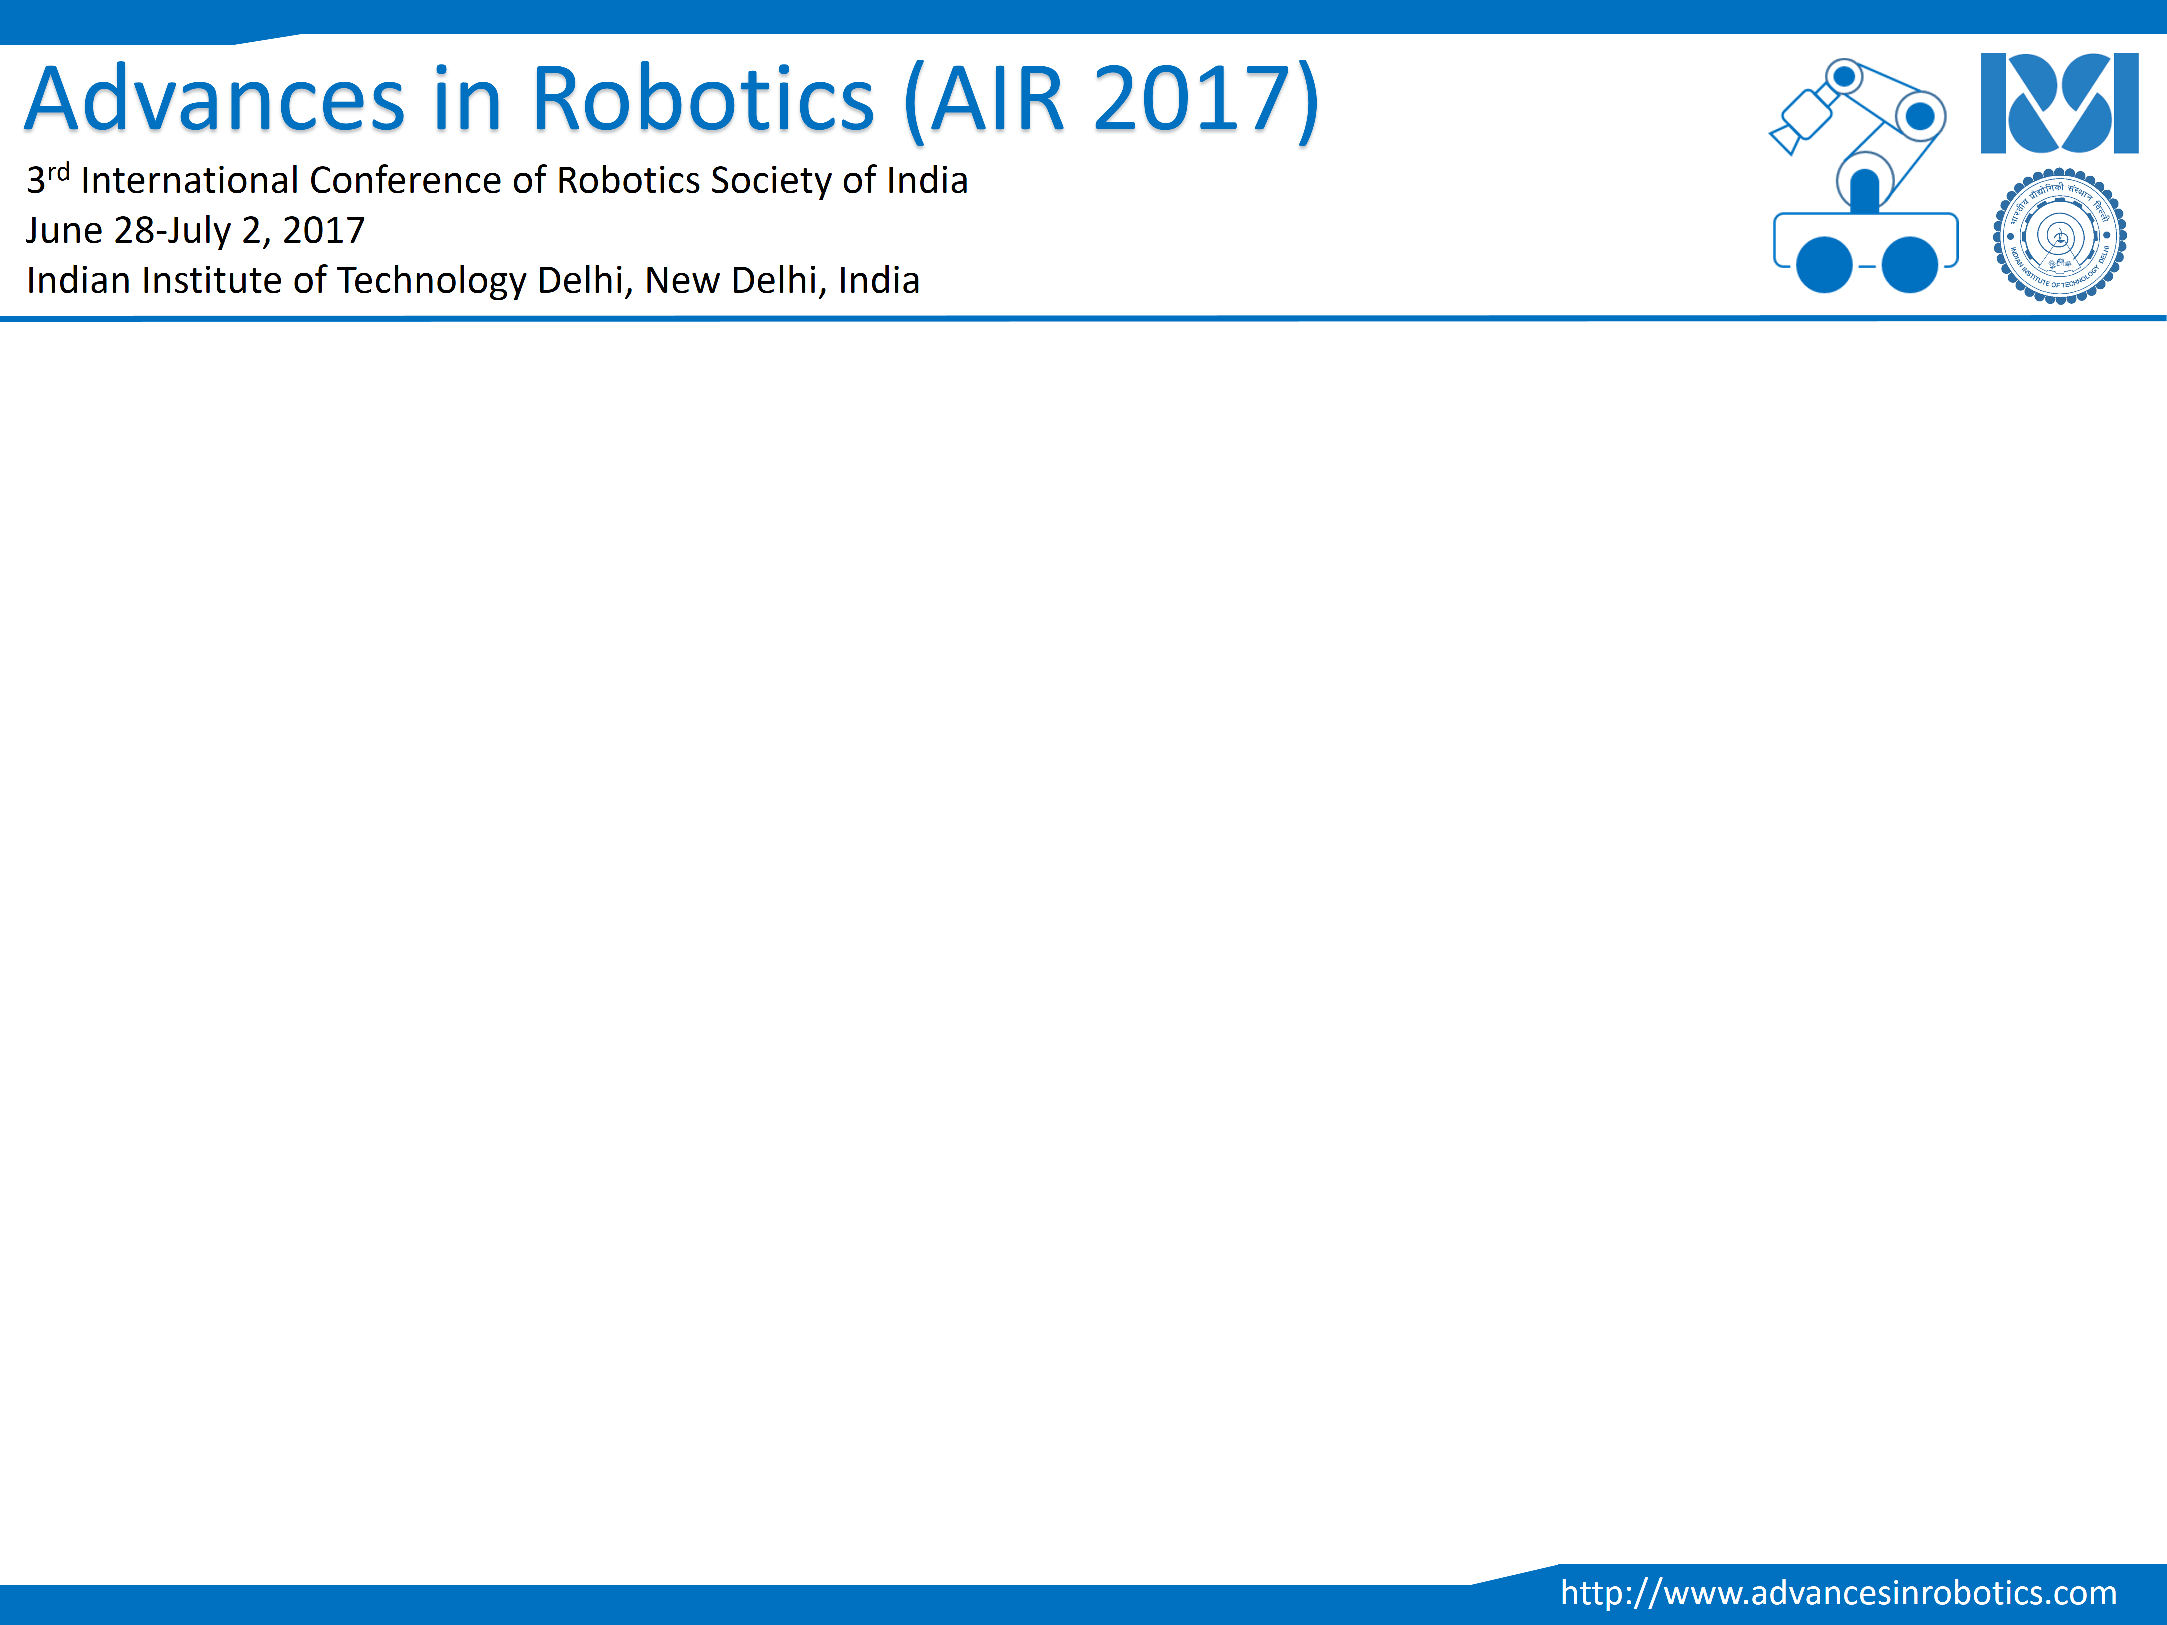
\includegraphics[width=\paperwidth]{background.pdf}}
  \setbeamertemplate{footline}{} 
  \begin{frame}
    \titlepage
  \end{frame}
}
\addtocounter{framenumber}{-1}

%\begin{frame}[noframenumbering]
%	\titlepage
%\end{frame}

\begin{frame}[noframenumbering]{Outline}
	\tableofcontents
\end{frame}

\section{Introduction}
\begin{frame}{Introduction}
	\linespread{1.6}
		
	\begin{itemize}
		\item Clothing assistance is a basic and important assistance activity in the daily life of the elderly and disabled people
		\item Need of robotic clothing assistance is growing
	\end{itemize}
		
	\vskip 1em
	\begin{block}{Major challenges involved}
		\begin{itemize}
			\item Close interaction of the robot with non-rigid clothing article
			\item Safe human-robot interaction
			\item Accurate estimation of human-cloth relationship
		\end{itemize}
	\end{block}
\end{frame}

\section{Related Works}
\begin{frame}{Related Works}
		
	\vskip -1em
	\begin{columns}[t]
		\begin{column}{0.5\textwidth}
			Towner \textit{et al.}\footnotemark, ~Identifying and manipulating clothing article by dual-arm robot
			{\scriptsize
				\begin{itemize}
					\item[\color{green}{\checkmark}] Used Hidden Markov Model for tracking
					\item[\color{green}{\checkmark}] Triangulated mesh model for simulating clothing article
					\item[\color{red}{$\times$}] Simple manipulations such as gripping using one arm only
				\end{itemize}
			}
			\vskip 0.5em
			\centering{
				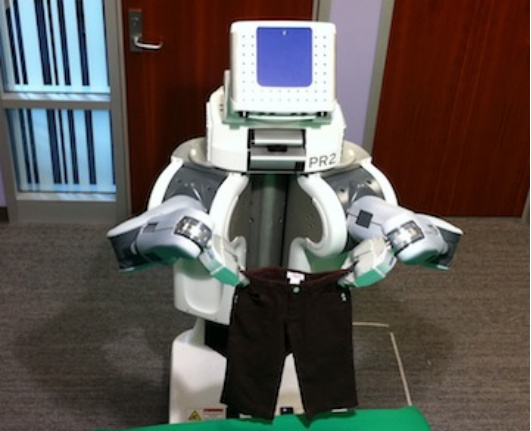
\includegraphics[height=2.5cm]{towner_2011}
			}
		\end{column}
				
		\begin{column}{0.5\textwidth}
			Tamei \textit{et al.}\footnotemark, ~Clothing assistance with dual-arm robot
			{\scriptsize
				\begin{itemize}
					\item[\color{green}{\checkmark}] Used Reinforcement
					      learning (RL)
					\item[\color{green}{\checkmark}] Topology coordinates for human and cloth extremities relationship
					\item[\color{red}{$\times$}] Limited generalization capability for new postures
				\end{itemize}
			}
			\vskip 0.5em
			\centering{
				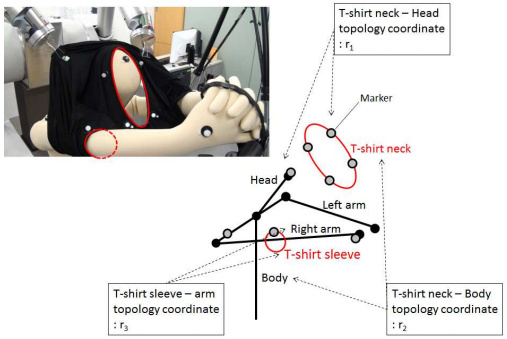
\includegraphics[height=2.5cm]{tamei_2011}
			}
		\end{column}
	\end{columns}
		
	\addtocounter{footnote}{-1}
	\footcitetext{cusumano2011bringing}
	\stepcounter{footnote}
	\footcitetext{tamei2011reinforcement}
\end{frame}

\section{Dynamic Movement Primitives}
\begin{frame}{Dynamic Movement Primitives (DMP)}
	%\linespread{1.2}
		
	\begin{exampleblock}{DMP in a nutshell}
		\begin{itemize}
			\item It is used for generating a control signal to guide the real system\footnotemark
			\item It can represent \textit{nonlinear} motion with a set of differential equations
		\end{itemize}
	\end{exampleblock}
		
		
	%	We start with point attractor dynamics\footcite{ijspeert2002movement} \hskip1em $\ddot{y} = \alpha_y ( \beta_y (g - y) - \dot{y})$
		
	%	\vskip -1em
	%	\begin{equation}
	%		\ddot{y} = \alpha_y ( \beta_y (g - y) - \dot{y})
	%		\label{eq:attractor}
	%	\end{equation}
	%	\vskip -0.5em
		
	%	\vskip 1em
	%	Now add a forcing term $f$ on eq(\ref{eq:attractor}) that will let us to modify this trajectory
	The system is defined as
	\vskip -1em
	\begin{equation}
		\ddot{y} = \alpha_y ( \beta_y (g - y) - \dot{y}) + f
		\label{eq:attractor_with_f}
	\end{equation}
	%\vskip -0.5em
	{\small
		where:
		\vskip -0.6em
		\begin{itemize}
			\itemsep-0.2em
			\item $y$ is system state and $g$ is goal state
			\item $\alpha$ and $\beta$ are gain terms
			\item $f$ is nonlinear function defined over time
		\end{itemize}
	}
		
	\begin{exampleblock}{}
		$f$ is a function of \textit{canonical system}, denoted by $x$ as $\dot{x} = -\alpha_x x$
	\end{exampleblock}
		
	\footcitetext{schaal2006dynamic}
\end{frame}


\begin{frame}{Forcing function $f$}
	$f$ is defined as
	\begin{equation}
		f(x,g) = \frac{\Sigma_{i=1}^N \psi_i w_i}{\Sigma_{i=1}^N \psi_i} x(g - y_0)
		\label{eq:cs_with_f}
	\end{equation}
		
	where:
	\begin{itemize}
		\item $y_0$ is the initial state of the system
		\item $w_i$ is a weighting for a given basis function $\psi_i$
		\item $\psi_i = \textrm{exp}\left( -h_i \left( x - c_i\right)^2 \right)$ is Gaussian with mean $c_i$ and variance $h_i$
	\end{itemize}
		
	\vskip -1em
	\begin{columns}
		\begin{column}{0.5\textwidth}
			\begin{figure}
				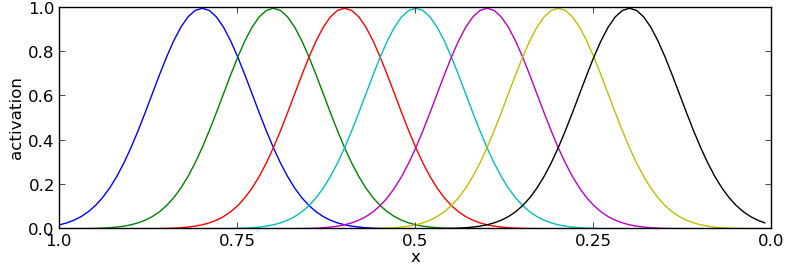
\includegraphics[height=2.1cm]{psi_activation}
				\vskip -0.3em
				\caption{$\psi$ Activation}
			\end{figure}
		\end{column}
				
		\begin{column}{0.5\textwidth}
			\begin{figure}
				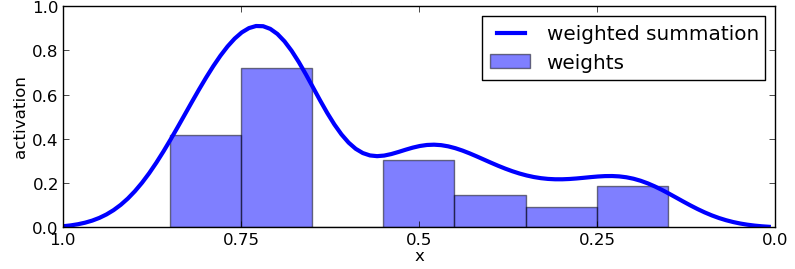
\includegraphics[height=2.1cm]{weighted_summation}
				\vskip -0.3em
				\caption{Weighted Summation}
			\end{figure}
		\end{column}
	\end{columns}
\end{frame}

\begin{frame}{Imitating a desired path}
	\linespread{1.4}
	The desired forcing term $f$ which affects the system acceleration, is written as
	\vskip -1.5em
	\begin{equation}
		\textbf{f}_d = \ddot{\textbf{y}}_d - \alpha_y ( \beta_y (g - \textbf{y}) - \dot{\textbf{y}})
		\label{eq:imitate_f}
	\end{equation}
	\vskip -0.5em
	{\small
		where 
		\vskip -1em
		\begin{itemize}
			\item $\textbf{y}_d$ is desired trajectory, given by $\ddot{\textbf{y}}_d = \frac{\partial}{\partial t} \dot{\textbf{y}}_d = \frac{\partial}{\partial t} \frac{\partial}{\partial t} \textbf{y}_d$
		\end{itemize}
	}
	\vskip-0.5em
	\begin{exampleblock}{}
		Choose the weights over the basis functions i.e., minimize\footnotemark
		\vskip-2em
		\begin{equation}
			\Sigma_t \psi_i(t) \left[ f_d(t) - w_i \left\lbrace x(t) (g - y_0)\right\rbrace\right]^2
			\label{eq:minize_fd}
		\end{equation}
	\end{exampleblock}
	\vskip-0.5em
	\begin{figure}
		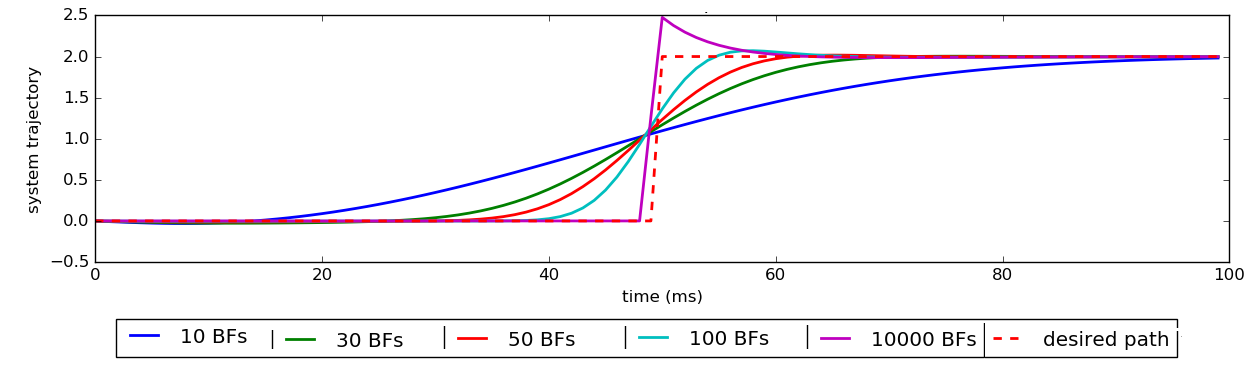
\includegraphics[width=0.8\textwidth]{imitate_path}
	\end{figure}
	\vskip-1.5em
	\footcitetext{schaal2002scalable}
\end{frame}

\section{Setup and Experiment}
\begin{frame}{Workflow of \textit{Robotic cloth manipulation} task}
	\vskip -0.5em
	\begin{figure}
		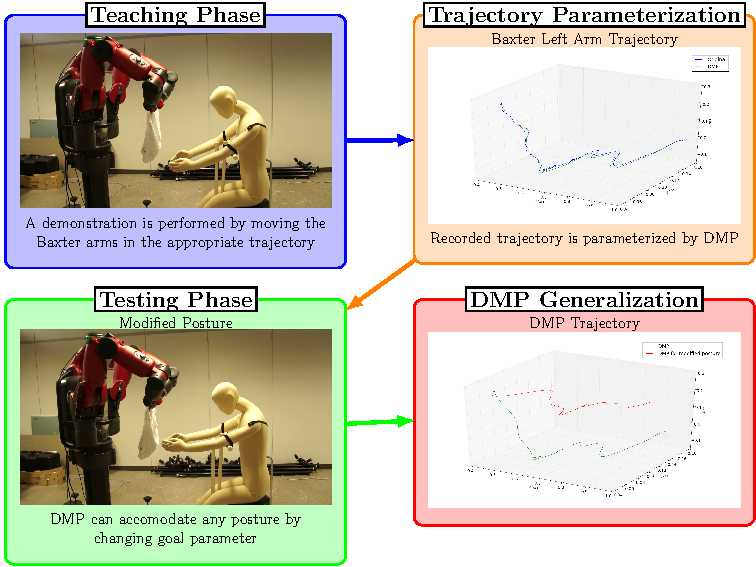
\includegraphics[width=0.85\textwidth]{flowchart_beamer_hd}
	\end{figure}
\end{frame}

\begin{frame}{Setup}
	\begin{figure}
		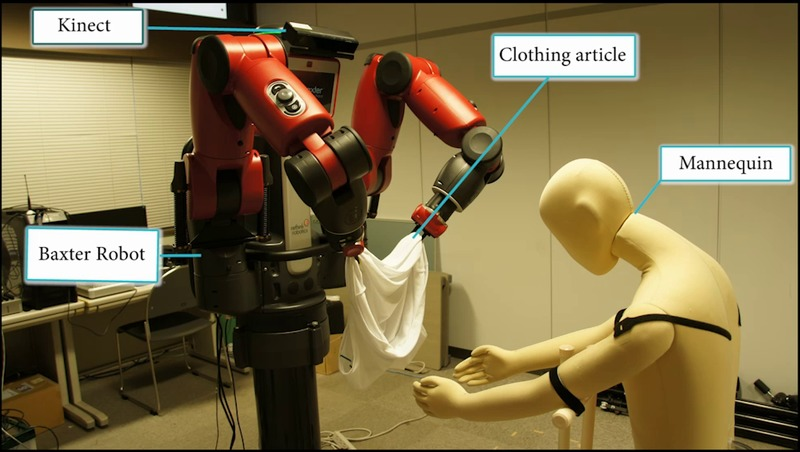
\includegraphics[width=\textwidth]{setup}
	\end{figure}
\end{frame}

\section{Results}
\begin{frame}{Results}
	\begin{columns}[b]
		\begin{column}{0.5\textwidth}
			\begin{figure}
				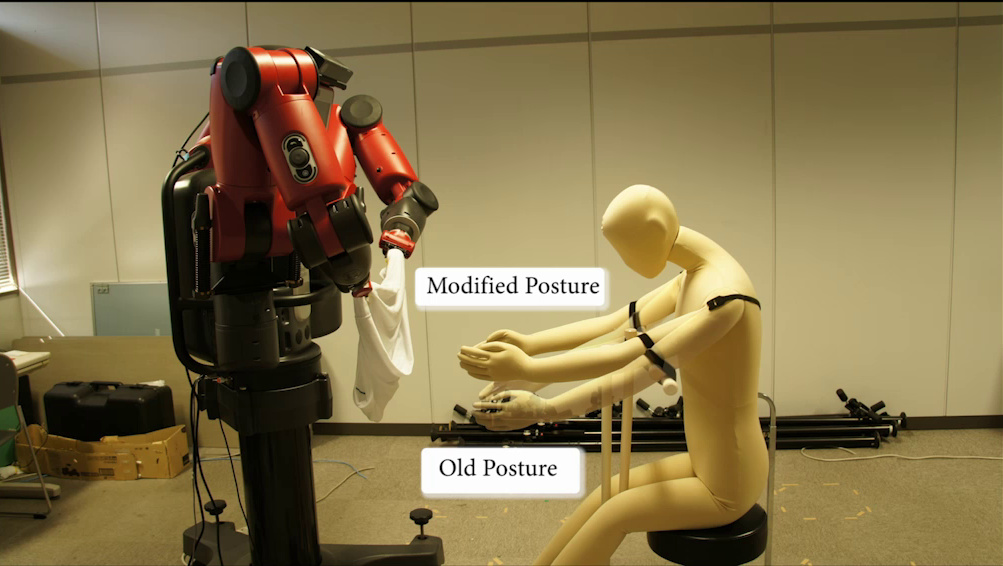
\includegraphics[width=\textwidth]{various_posture}
				\caption{Old \& modified posture of mannequin}
			\end{figure}
		\end{column}
				
		\begin{column}{0.5\textwidth}
			\begin{figure}
				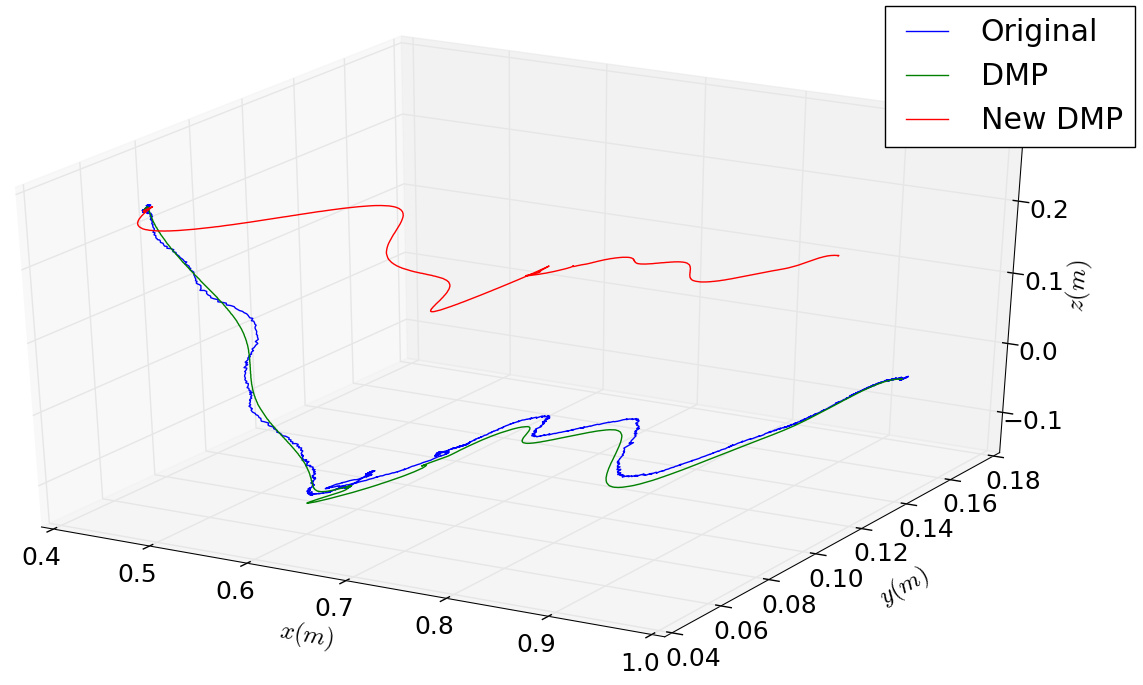
\includegraphics[width=\textwidth]{trajectory}
				\caption{Left arm trajectories of Baxter Robot}
			\end{figure}
		\end{column}
	\end{columns}
		
	\vskip 1em
	\centering{
		\href{run:./videos/video.mp4}{\beamerbutton{Video demonstration}}
	}
\end{frame}

\section{Conclusion and Discussion}
\begin{frame}{Conclusion and Discussion}
	\linespread{1.5}
		
	\begin{itemize}
		\item Result shows that DMPs are able to generalize the movement trajectory
		\item The converted trajectory from Cartesian Space to Joint Space was not smooth in some regions
		      \begin{itemize}
		      	\item It was calculated using \textsc{Trac\_IK}\footcite{beeson2015trac}
		      \end{itemize}
		\item Also real-time tracking of mannequin is required
	\end{itemize}
\end{frame}

\section{Future work}
\begin{frame}{Tentative Research Plan}
	
	\begin{figure}
		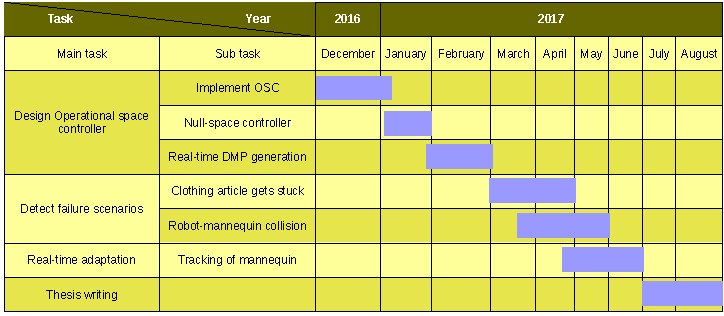
\includegraphics[width=\textwidth]{timeline}
	\end{figure}
\end{frame}

\begin{frame}[noframenumbering]{References}
	\nocite{*}
	\hspace*{0.5cm}
	\begin{minipage}{\dimexpr\textwidth-1cm\relax}
		\printbibliography
	\end{minipage}
\end{frame}



\begin{frame}[noframenumbering]{The End}
	\begin{center}
		\Huge Thanks for your attention!
		\vskip 1em \huge Any questions?
		\vskip 2em \normalsize \url{www.ravijoshi.xyz}
	\end{center}
\end{frame}

\end{document}
